\documentclass{article}
\usepackage{amsmath}
\usepackage{tikz}
\usetikzlibrary{matrix}
\usetikzlibrary{positioning}
\usetikzlibrary{patterns,patterns.meta}
\usetikzlibrary{shapes.geometric}
\pgfdeclarepatternformonly{south east lines}{\pgfqpoint{-0pt}{-0pt}}{\pgfqpoint{8pt}{8pt}}{\pgfqpoint{8pt}{8pt}}{
    \pgfsetlinewidth{0.4pt}
    \pgfpathmoveto{\pgfqpoint{0pt}{8pt}}
    \pgfpathlineto{\pgfqpoint{8pt}{0pt}}
    \pgfpathmoveto{\pgfqpoint{.2pt}{-.2pt}}
    \pgfpathlineto{\pgfqpoint{-.2pt}{.2pt}}
    \pgfpathmoveto{\pgfqpoint{8.2pt}{7.8pt}}
    \pgfpathlineto{\pgfqpoint{7.8pt}{8.2pt}}
    \pgfusepath{stroke}}

\begin{document}

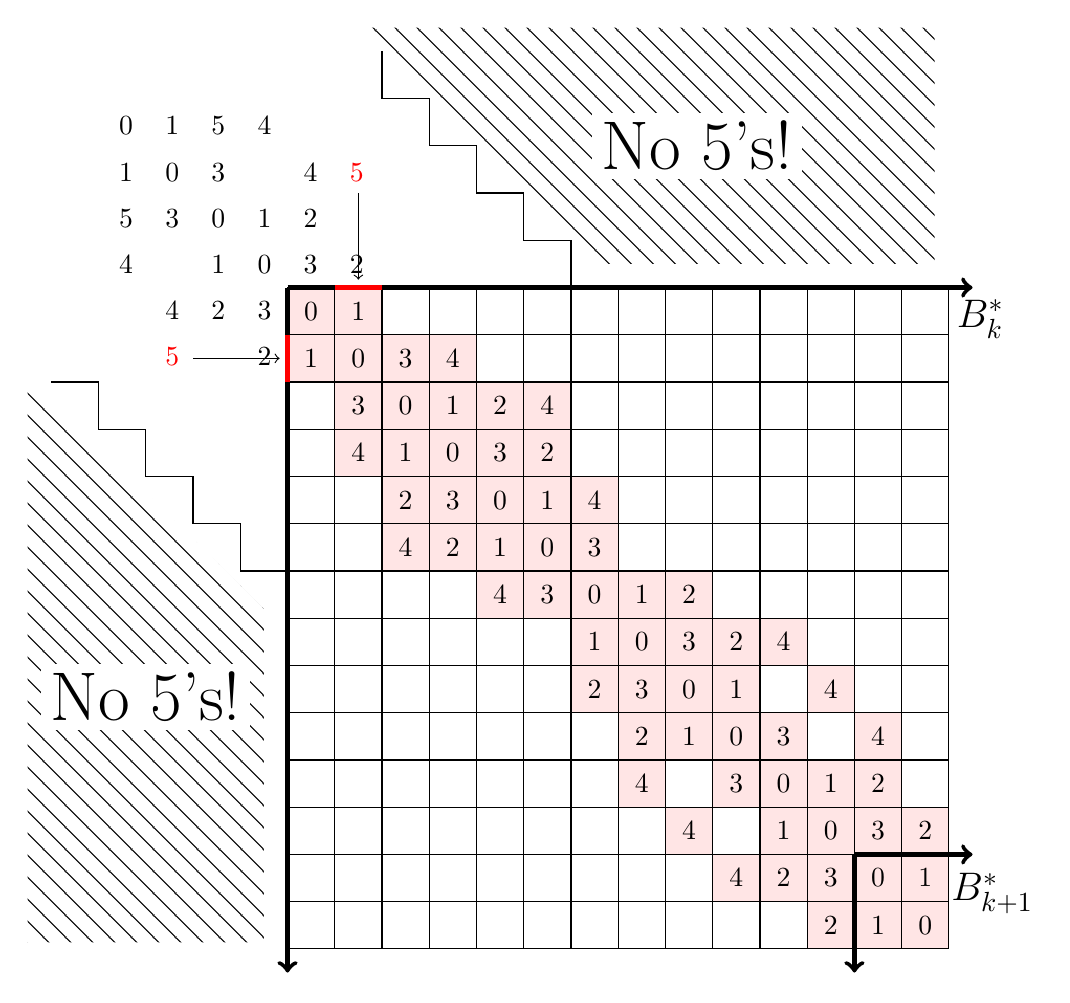
\begin{tikzpicture}[ne/.style={fill=red!10}]
    \matrix (main) at (0, 0) [matrix of nodes, nodes in empty cells, nodes={rectangle, minimum width=0.6cm, minimum height=0.6cm, anchor=center, draw}, row sep=-\pgflinewidth, column sep=-\pgflinewidth] {
        |[ne]| 0 & |[ne]| 1 & & & & & & & & & & & & \\
        |[ne]| 1 & |[ne]| 0 & |[ne]| 3 & |[ne]| 4 & & & & & & & & & & \\
        & |[ne]| 3 & |[ne]| 0 & |[ne]| 1 & |[ne]| 2 & |[ne]| 4 &&&&&&&&\\
        & |[ne]| 4 & |[ne]| 1 & |[ne]| 0 & |[ne]| 3 & |[ne]| 2 &&&&&&&&\\
        && |[ne]| 2 & |[ne]| 3 & |[ne]| 0 & |[ne]| 1 & |[ne]| 4 &&&&&&&\\
        && |[ne]| 4 & |[ne]| 2 & |[ne]| 1 & |[ne]| 0 & |[ne]| 3 &&&&&&&\\
        &&&& |[ne]| 4 & |[ne]| 3 & |[ne]| 0 & |[ne]| 1 & |[ne]| 2 &&&&&\\
        &&&&&& |[ne]| 1 & |[ne]| 0 & |[ne]| 3 & |[ne]| 2 & |[ne]| 4 &&&\\
        &&&&&& |[ne]| 2 & |[ne]| 3 & |[ne]| 0 & |[ne]| 1 & & |[ne]| 4 &&\\
        &&&&&&& |[ne]| 2 & |[ne]| 1 & |[ne]| 0 & |[ne]| 3 & & |[ne]| 4 &\\
        &&&&&&& |[ne]| 4 & & |[ne]| 3 & |[ne]| 0 & |[ne]| 1 & |[ne]| 2 &\\
        &&&&&&&& |[ne]| 4 & & |[ne]| 1 & |[ne]| 0 & |[ne]|3 & |[ne]| 2 \\
        &&&&&&&&& |[ne]| 4 & |[ne]| 2 & |[ne]| 3 & |[ne]| 0 & |[ne]| 1 \\
        &&&&&&&&&&& |[ne]| 2 & |[ne]| 1 & |[ne]| 0 \\
    };

    \draw[ultra thick] (-4.2, 4.2)--(-4.2, 3.6);
    \draw[ultra thick, color=red] (-4.2, 3.6)--(-4.2, 3.0);
    \draw[ultra thick, ->] (-4.2, 3.0)--(-4.2, -4.5);
    \draw[ultra thick] (-4.2, 4.2)--(-3.6, 4.2);
    \draw[ultra thick, color=red] (-3.6, 4.2)--(-3, 4.2);
    \draw[ultra thick, ->] (-3, 4.2)--(4.5, 4.2);
    \node at (4.6, 3.8) {\Large $B^*_k$};

    \draw[ultra thick, ->] (3, -3)--(3, -4.5);
    \draw[ultra thick, ->] (3, -3)--(4.5, -3);
    \node at (4.75, -3.5) {\Large $B^*_{k+1}$};

    \draw (-0.6, 4.2)--(-0.6, 4.8)--(-1.2, 4.8)--(-1.2, 5.4)--(-1.8, 5.4)--(-1.8, 6)--(-2.4, 6)--(-2.4, 6.6)--(-3, 6.6)--(-3, 7.2);
    \draw (-4.2, 0.6)--(-4.8, 0.6)--(-4.8, 1.2)--(-5.4, 1.2)--(-5.4, 1.8)--(-6, 1.8)--(-6, 2.4)--(-6.6, 2.4)--(-6.6, 3)--(-7.2, 3);

    \node
    [
    trapezium, 
    trapezium left angle=125, 
    trapezium right angle=90, 
    trapezium stretches=true,
    minimum height=3cm,
    minimum width=7.2cm,
    pattern=south east lines
    ] at (1.9, 6) {};
    \node[fill=white] at (1, 6) {\Huge No 5's!};

    \node
    [
    trapezium, 
    trapezium left angle=90, 
    trapezium right angle=125, 
    trapezium stretches=true,
    minimum height=3cm,
    minimum width=7.2cm,
    rotate=90,
    pattern=south east lines
    ] at (-6, -2) {};
    \node[fill=white] at (-6, -1) {\Huge No 5's!};

    \matrix (upper) at (-4.2, 4.2) [matrix of nodes, nodes in empty cells, nodes={minimum width=0.6cm, minimum height=0.6cm, anchor=center}, row sep=-\pgflinewidth, column sep=-\pgflinewidth] {
        0 & 1 & 5 & 4 &   &   &   &   \\
        1 & 0 & 3 &   & 4 & |[color=red]| 5 &   &   \\
        5 & 3 & 0 & 1 & 2 &   &   &   \\
        4 &   & 1 & 0 & 3 & 2 &   &   \\
          & 4 & 2 & 3 &   &   &   &   \\
          & |[color=red]| 5 &   & 2 &   &   &   &   \\
          &   &   &   &   &   &   &   \\
          &   &   &   &   &   &   &   \\
    };

    \draw[->] (-5.4, 3.3)--(-4.3, 3.3);
    \draw[->] (-3.3, 5.4)--(-3.3, 4.3);
\end{tikzpicture}

\end{document}